%! Tex program = xelatex
\documentclass{article}
%中文
%\usepackage[UTF8]{ctex}
%数学公式
\usepackage{amsmath,amssymb}
%\usepackage{ntheorem}
\usepackage{amsthm}
%边界
\usepackage[letterpaper,top=1cm,bottom=2cm,left=3cm,right=3cm,marginparwidth=1.75cm]{geometry}%table package
%Table
\usepackage{multirow,booktabs}
\usepackage{makecell}
%字体颜色
\usepackage{color}
\usepackage[dvipsnames]{xcolor}  % 更全的色系
%代码
\usepackage[OT1]{fontenc}
% MATLAB 代码风格
\usepackage[framed,numbered,autolinebreaks,useliterate]{/Users/anye_zhenhaoyu/Desktop/Latex/mcode}
\usepackage{listings}
\usepackage{algorithm}
\usepackage{algorithmic}
\usepackage{pythonhighlight} % Python
%插图
\usepackage{graphicx}
%改变item格式
\usepackage{enumerate}
%物理
\usepackage{physics}
%extra arrows
\usepackage{extarrows}
% caption(居中指令)
%\usepackage[justification=centering]{caption}
\usepackage{caption}
% htpb
\usepackage{stfloats}
% pdf 拼接
\usepackage{pdfpages}
% 超链接url
\usepackage{url}

\def\RR{\mathbb{R}}
\def\ZZ{\mathbb{Z}}
\def\EE{\mathbb{E}}

\def\Trsp#1{#1^{\mathcal{T}}}
\def\LT{\mathcal{L}}

\def\bold#1{\boldsymbol{#1}}
\def\bw{\boldsymbol{\omega}}
\def\ba{\boldsymbol{a}}
\def\bb{\boldsymbol{b}}
\def\bc{\boldsymbol{c}}
\def\bd{\boldsymbol{d}}
\def\be{\boldsymbol{e}}
\def\bf{\boldsymbol{f}}
\def\bg{\boldsymbol{g}}
\def\bt{\boldsymbol{t}}
\def\bu{\boldsymbol{u}}
\def\bv{\boldsymbol{v}}
\def\bx{\boldsymbol{x}}
\def\by{\boldsymbol{y}}
\def\bz{\boldsymbol{z}}

\def\bA{\boldsymbol{A}}
\def\bB{\boldsymbol{B}}
\def\bC{\boldsymbol{C}}
\def\bE{\boldsymbol{E}}
\def\bL{\boldsymbol{L}}
\def\bM{\boldsymbol{M}}
\def\bO{\boldsymbol{O}}
\def\bP{\boldsymbol{P}}
\def\bQ{\boldsymbol{Q}}
\def\bX{\boldsymbol{X}}
\def\bY{\boldsymbol{Y}}

\def\Esolve{\textcolor{blue}{Solve: }}
\def\Eproof{\textcolor{blue}{Proof: }}
\def\case#1{\textcolor{blue}{Case \uppercase\expandafter{\romannumeral#1}: }}

\def\suminf#1{\sum_{#1=-\infty}^{+\infty}}

\newtheorem{lemma}{Lemma}
\newtheorem{theorem}{Theorem}
\newtheorem{defination}{Definition} 

\graphicspath{{figures/}}

\begin{document}
\title{Homework 11}
\author{Zhen}
\maketitle

\section*{Problem 1}
\begin{python}
def proj(x):
	if np.linalg.norm(x,1)<1:
		return x
	k = x / np.abs(x)
	c = (t - k.T @ x) / (np.linalg.norm(k)**2)
	x = c * k + x
	return x
\end{python}
The implementation of the projection onto $l_1$ ball is above. Let the stepsize$=0.1$. The output is:
\\
\texttt{
t =  1\\
number of iterations: 122\\
solution: [9.99999975e-01 2.51943348e-08]\\
value: 4.500000000000001
}
\\
Some useful plots:
\begin{figure}[H]
	\centering
	\begin{minipage}[b]{0.46\linewidth}
		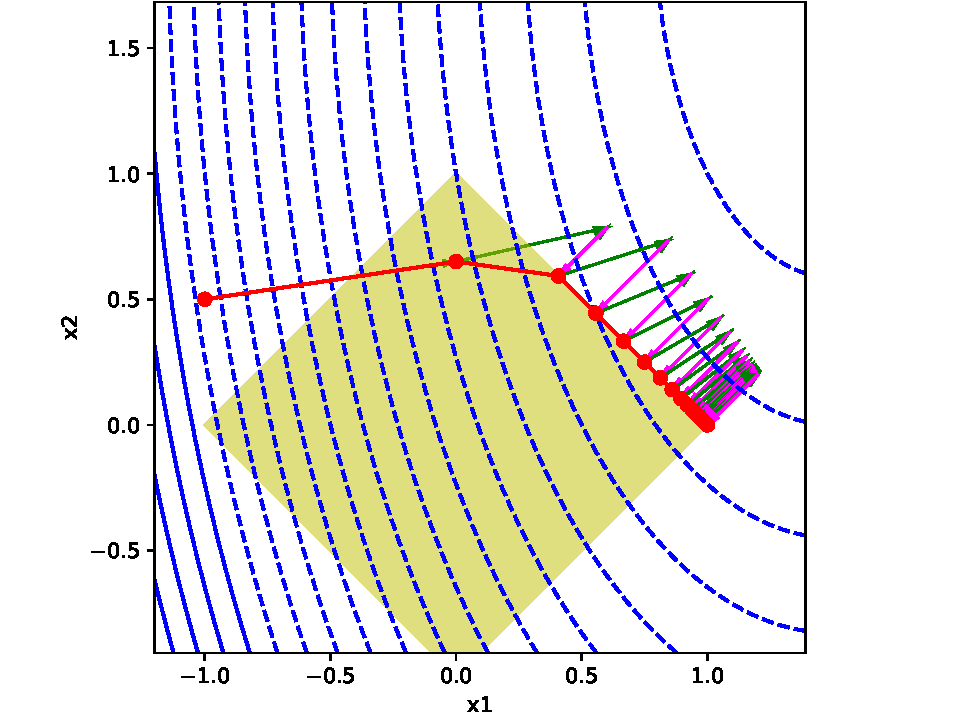
\includegraphics[width=\linewidth]
		{lasso_traces_t1.pdf}
		\caption{the trajectory of $\bx_k$}
	\end{minipage}
	\begin{minipage}[b]{0.46\linewidth}
		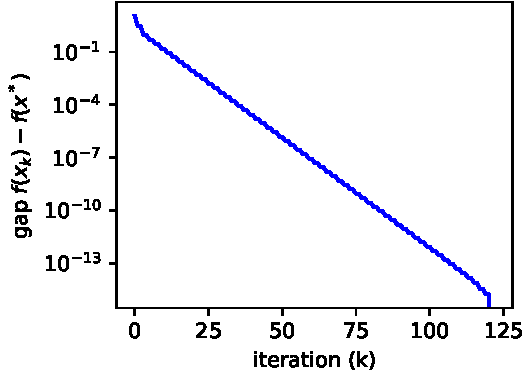
\includegraphics[width=\linewidth]
		{lasso_gap_t1.pdf}
		\caption{the gap $f(\bx_k) - f(\bx^*)$}
	\end{minipage}
\end{figure}

\newpage
\section*{Problem 2}

\begin{enumerate}[(a)]
    \item
		The Lagrangian condition is:
		\[
		    \begin{aligned}
		        &x_1+x_2+x_3=1 \\
				&e^{x_1}+\lambda=0 \\
				&2e^{2x_2}+\lambda=0 \\
				&2e^{2x_3}+\lambda=0 \\
		    \end{aligned}
		\]
		Then we have:
		\[
			x_1=\ln(-\lambda),\ \ 
			x_2=x_3=\frac{1}{2}\ln(-\frac{\lambda}{2})
		\]
		Thus we have: 
		$
		\lambda^*=-\sqrt{2e},
		\bx^*=\mqty[\ln(\sqrt{2e}) & \dfrac{1}{2}\ln(\sqrt{2e}/2) & \dfrac{1}{2}\ln(\sqrt{2e}/2)]
		$
		and $f^*=-2\lambda=2\sqrt{2e}$.
    \item
		Similarly, let the stepsize$=0.1$. The output is:\\
		\texttt{
			number of iterations: 92 \\
			solution: [0.84657357 0.07671322 0.07671322] \\
			value: 4.66328796319425
		}\\
		which is in accord with theoretical value.
\end{enumerate}


\end{document}

